\subsection{Sub Unit}
\subsubsection{Block Diagram}
\createfigurewsvg{../Modular Design/Sub-Unit/Figures/bdv5-sub.svg}{Sub Unit Architectural Diagram}{fig:bd-module-sub-unit}
\subsubsection{State Diagram}
\begin{landscape}
\begin{figure}[!ht]
\begin{center}
  \begin{subfigure}{\textwidth}
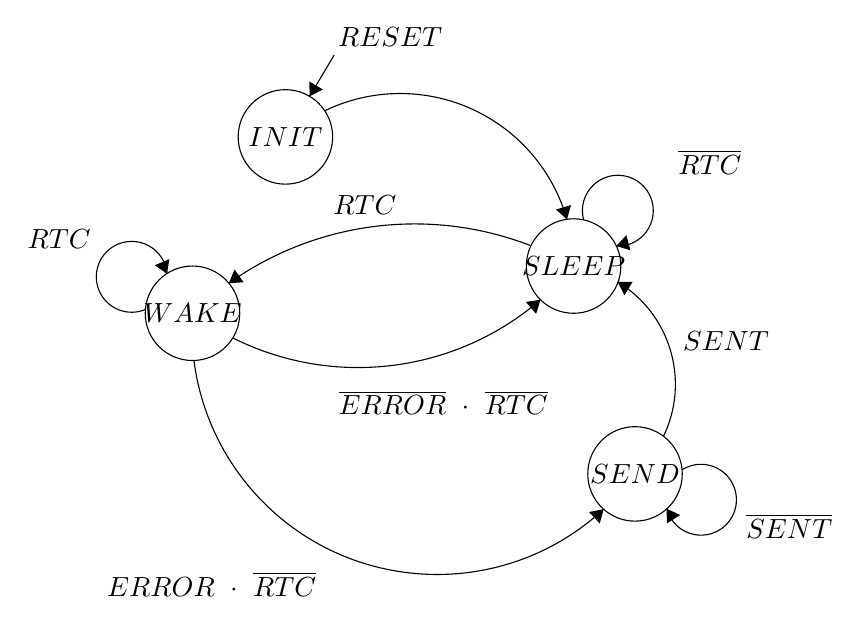
\begin{tikzpicture}[scale=0.2]
\tikzstyle{every node}+=[inner sep=0pt]
\draw [black] (36.8,-8) circle (3);
\draw (36.8,-8) node {$INIT$};
\draw [black] (55.1,-16.2) circle (3);
\draw (55.1,-16.2) node {$SLEEP$};
\draw [black] (30.9,-19.2) circle (3);
\draw (30.9,-19.2) node {$WAKE$};
\draw [black] (59,-29.4) circle (3);
\draw (59,-29.4) node {$SEND$};
\draw [black] (39.9,-2.8) -- (38.34,-5.42);
\draw (43.45,-2.3) node [above] {$RESET$};
\fill [black] (38.34,-5.42) -- (39.18,-4.99) -- (38.32,-4.48);
\draw [black] (39.29,-6.344) arc (115.82686:15.90003:11.012);
\fill [black] (54.68,-13.24) -- (54.94,-12.33) -- (53.98,-12.61);
\draw [black] (55.741,-13.281) arc (195.34019:-92.65981:2.25);
\draw (63.76,-10.43) node [above] {$\overline{RTC}$};
\fill [black] (57.81,-14.93) -- (58.71,-15.2) -- (58.45,-14.24);
\draw [black] (33.209,-17.289) arc (125.38493:68.74853:20.376);
\fill [black] (33.21,-17.29) -- (34.15,-17.23) -- (33.57,-16.42);
\draw (41.85,-12.97) node [above] {$RTC$};
\draw [black] (57.903,-17.214) arc (58.79222:-25.87219:7.596);
\fill [black] (57.9,-17.21) -- (58.33,-18.06) -- (58.85,-17.2);
\draw (62.02,-20.97) node [right] {$SENT$};
\draw [black] (53.003,-18.341) arc (-49.24761:-116.61893:17.757);
\fill [black] (53,-18.34) -- (52.07,-18.48) -- (52.72,-19.24);
\draw (46.82,-24.07) node [below] {$\overline{ERROR}\mbox{ }\cdot\mbox{ }\overline{RTC}$};
\draw [black] (57.009,-31.638) arc (-47.17822:-172.72249:15.564);
\fill [black] (57.01,-31.64) -- (56.08,-31.82) -- (56.76,-32.55);
\draw (32.12,-35.61) node [below] {$ERROR\mbox{ }\cdot\mbox{ }\overline{RTC}$};
\draw [black] (61.977,-29.145) arc (122.62938:-165.37062:2.25);
\draw (66.04,-32.72) node [right] {$\overline{SENT}$};
\fill [black] (61.01,-31.61) -- (61.02,-32.55) -- (61.87,-32.01);
\draw [black] (27.922,-18.955) arc (293.03624:5.03624:2.25);
\draw (24.47,-14.46) node [left] {$RTC$};
\fill [black] (29.28,-16.69) -- (29.43,-15.76) -- (28.51,-16.15);
\end{tikzpicture}
\caption{Sub Unit Functional State Diagram}
\label{fig:sub-unit-fsd-diagram}
  \end{subfigure}
  \begin{subfigure}[b]{0.5\textwidth}
      \begin{tabular}{c|cccc}
        STATE&\multicolumn{3}{c}{OUTPUTS}\\
        \hline
        &&&\\
        INIT&$RESET$&$\overline{RTC}$&$\overline{SENT}$&$\overline{ERROR}$\\
        SLEEP&$\overline{RESET}$&$\overline{RTC}$&$\overline{SENT}$&$\overline{ERROR}$\\
        WAKE&$\overline{RESET}$&$RTC$&$\overline{SENT}$&$\overline{ERROR}$\\
        SEND&$\overline{RESET}$&$\overline{RTC}$&$\overline{SENT}$&$ERROR$\\
      \end{tabular}
      \caption{Sub Unit Functional State Diagram: State and Outputs}
      \label{fig:sub-unit-fsd-state-outputs}
  \end{subfigure}
  \begin{subfigure}[b]{0.5\textwidth}
   \begin{tabular}{|c|}
    \hline
     Output List\\
    \hline
     RESET = Power on Reset\\
     SLEEP = MCU is in LPM4\\
     WAKE = RTC Timer turned on MCU\\
     SEND = Bluetooth module is sending data\\
     ERROR = Temperature or Age Related Error Detected\\
    \hline
   \end{tabular}
      \caption{Sub Unit Functional State Diagram: Output List}
      \label{fig:sub-unit-fsd-outputs-list}
  \end{subfigure}
\caption{Sub Unit Functional State Diagram}
\label{fig:sub-unit-fsd}
\end{center}
\end{figure}

\subsubsection{Schematic Diagram}
  \begin{center}
  \begin{figure}[H]
    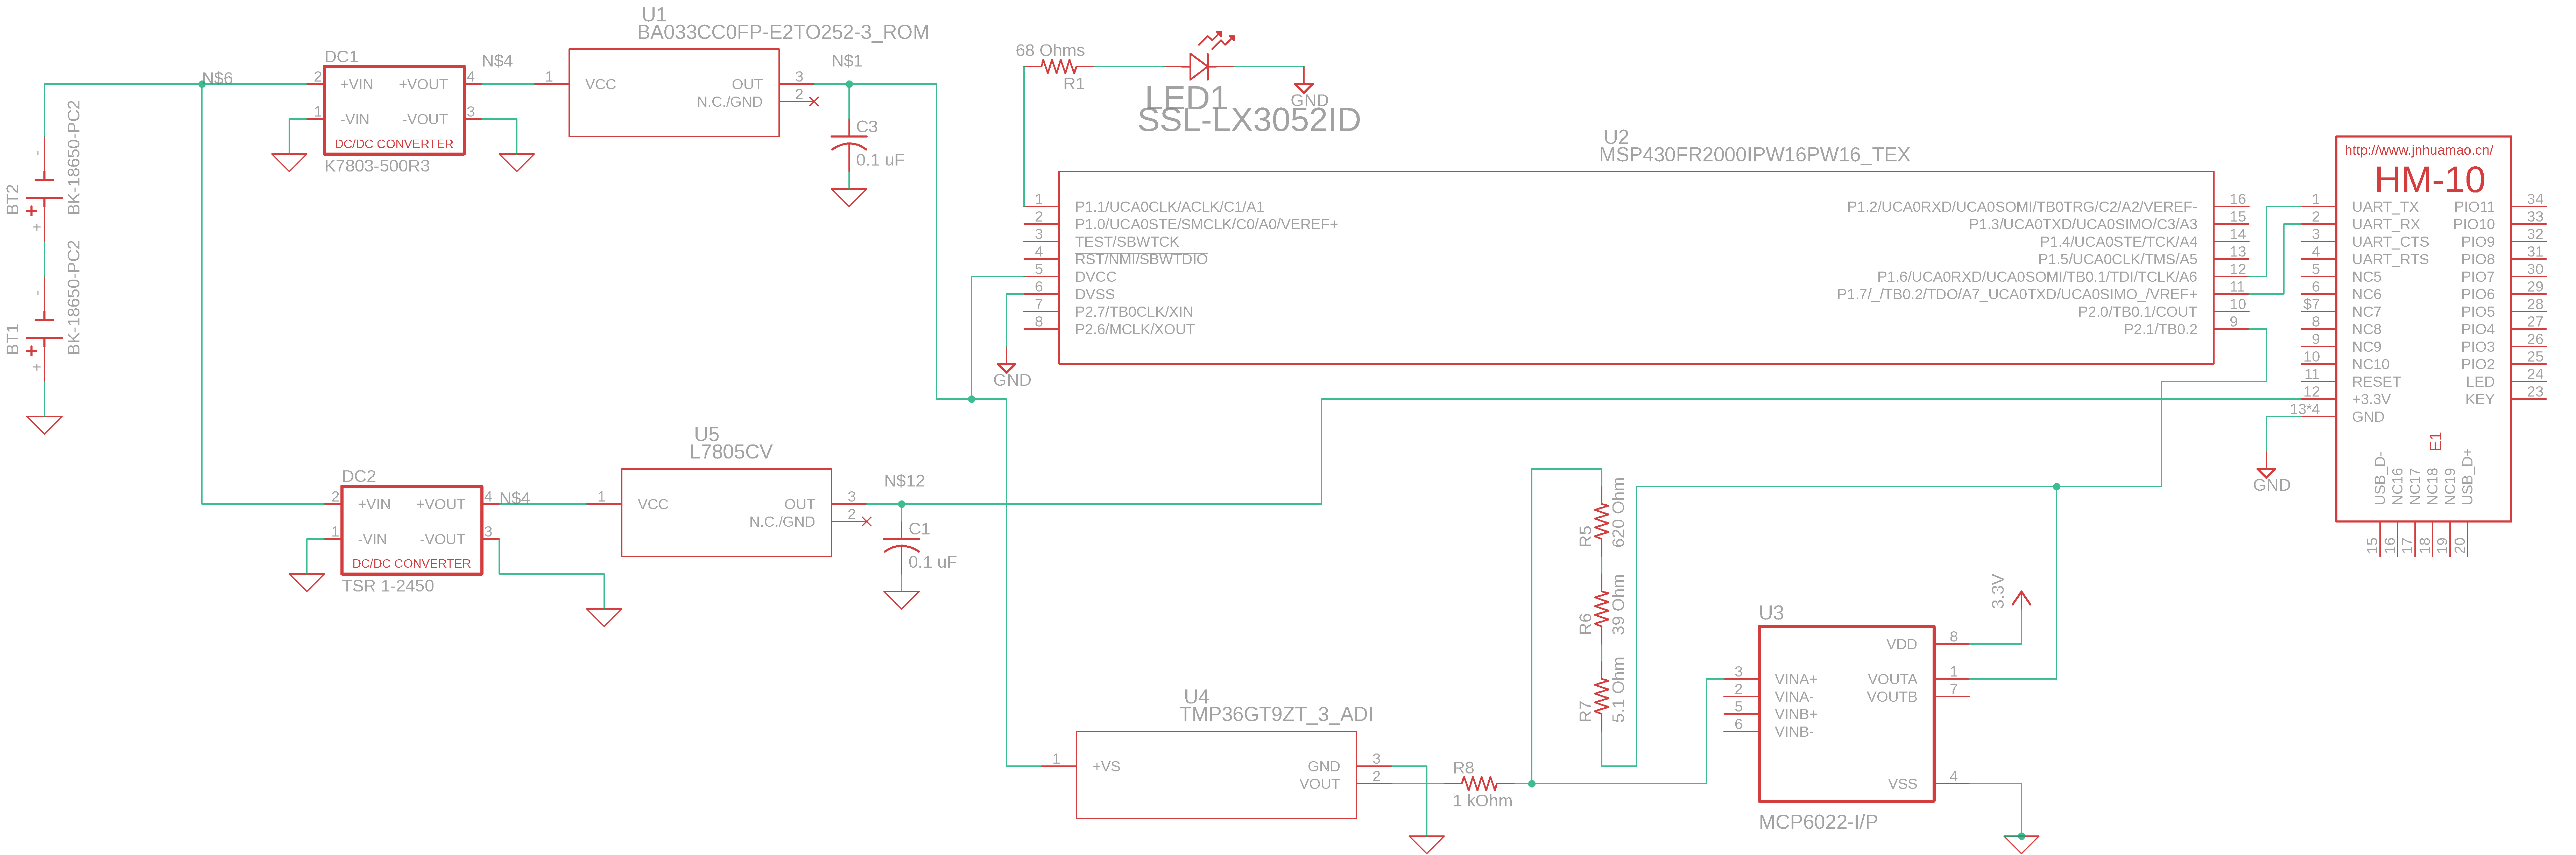
\includegraphics[width=\pdfpagewidth,height=0.65\textheight]{../Modular Design/Sub-Unit/Figures/sub-unit-and-psu.png}
    \caption{Sub Unit with PSU Schematic}
    \label{fig:sub-with-psu-schematic}
  \end{figure}
  \end{center}
  \end{landscape}
\subsubsection{Power Analysis, Loading, Driving, and Compatibility}
In order to validate the compatibility of the MCU (MSP430FR2000IPW16) and Bluetooth module (HM-10S) with respect to their voltage levels and communication protocols, it is necessary to verify their respective related specifications.\\
The MSP430FR2000IPW16 showcases flexibility in terms of voltage adaptability, functioning within a supply range ranging from 1.8V to 3.6V as seen in page 1 of its data sheet \cite{MSP430FR2000IPW16}. On the other hand, the HM-10 Bluetooth module has an input voltage from 3.6\si{\V} to 6\si{\V} according to it's product listing \cite{AmazonComHiLetgo}. Due to this the MSP430FR2110 has to be supplied by the 3.3\si{V} output of the PSU and the HM-10 has to be supplied by the 5\si{\V} output of the power supply.\\
In order to connect both devices to each other, for communication, the best protocol to use will be UART. The MSP430FR2000 has 4 pins for UART communication using the eUSCI modules, which can detect automatically the baud-rate to be used. According to the datasheet for the HM-10 module\cite{AmazonComHiLetgo}, it can select the baud-rate to be used, which ranges from a minimum 1200 to a maximum of 230400. In the datasheet of the MSP430FR2000, the eUSCI clock frequency, UART mode, can reach a maximum of 5MHz, which means it can reach the maximum baud-rate of the Bluetooth module and can also select lower baud-rates, according to the formula:
\begin{equation}
	Clk Frequency = Baudrate \cdot 16
\end{equation}
This means if we select the maximum baud-rate of the HM-10 module, which is 230400, using the formula, we would need a frequency of 3.68MHz, which is still below the maximum frequency the eUSCI module on the MSP430FR2000. This will allow us to be able to use the HM-10 communicate via UART with the MSP430FR2000.\\
In order to calculate the resistor values for the green and red LEDs we used the following formula:
\begin{equation}
R = \frac{V_{cc} - V_{f}}{I_{f}}
\end{equation}
Where VCC is 3.3\si{\V} $V_{f}$ is the forward voltage for each LED and $I_{f}$ is the forward current for each LED. For the RED LED \cite{SSLLX3052ID}, it has a 2\si{\V} forward voltage and the MSP430FR200 has a max I/O current of 2\si{\mA}, this gives us a resistor value of  650\si{\ohm} in order to drive this LED successfully and within MCU maximum parameters.\\
Finally, for the temperature sensor (U5) \cite{TMP36GT9Z} and operational amplifier (U4) \cite{MCP6022I}, they both can be supplied by a 3.3\si{\V} supply and thus are compatible. Since the temperature sensor range for this application will be from 0\si{\celsius} to 40\si{\celsius}, at a resolution of 0.1\si{\celsius}, since there is an offset of 0.5\si{\V} by the temperature sensor gives us a range of 900 unique values so that the temperature sensor can reach its full negative temperature range. At 40\si{\celsius} the temperature sensor will be at 900\si{\milli\volt}, setting the ADC to use a 1.5\si{\V} reference. gives us a $A_{v}$ of 1.666. Setting up the op amp in a non inverting configuration, using 1\si{\kilo\ohm}, 620\si{\ohm}, 39\si{\ohm} and 5.1\si{\ohm} resistors will yield a $A_{v}$ of 1.6642.
\subsubsection{Base Times and Timing Analysis}
In order to connect both devices to each other, for communication, the best protocol to use will be UART. The MSP430FR2000 has 4 pins for UART communication using the eUSCI modules, which can detect automatically the baud-rate to be used. According to the datasheet for the HM-10 module\cite{AmazonComHiLetgo}, it can select the baud-rate to be used, which ranges from a minimum 1200 to a maximum of 230400. In the datasheet of the MSP430FR2000, the eUSCI clock frequency, UART mode, can reach a maximum of 5MHz, which means it can reach the maximum baud-rate of the Bluetooth module and can also select lower baud-rates, according to the formula:
\begin{equation}
	Clk Frequency = Baudrate \cdot 16
\end{equation}
This means if we select the maximum baud-rate of the HM-10 module, which is 230400, using the formula, we would need a frequency of 3.68MHz, which is still below the maximum frequency the eUSCI module on the MSP430FR2000. This will allow us to be able to use the HM-10 communicate via UART with the MSP430FR2000.\\
\subsubsection{Software Support}
\createfigurel{../Modular Design/Sub-Unit/Figures/sub-unit-main-function.png}{Sub Unit Main Function}{fig:sub-unit-main-function}
\createfigurel{../Modular Design/Sub-Unit/Figures/sub-unit-rtc-isr.png}{Sub Unit RTC ISR}{fig:sub-unit-rtc-isr}
This is the error verification subroutine that runs periodically, it first checks weather the temperature detected from the ADC is within 2\si{\celsius} to 8\si{\celsius}, if this check fails it determines which temperature range is detected. Then writes the LOT number and error code to the BTTXBUF and enables the UCTXIFG.
\createfigurew{../Modular Design/Sub-Unit/Figures/sub-unit-bluetooth-isr.png}{Sub Unit Bluetooth ISR}{fig:sub-unit-bluetooth-isr}
If the interrupt is from the receiver, it will write the incoming message to the BTRXBUF until the UART goes idle. If the interrupt is from the transmitter, it first checks weather the buffer has contents, if it does, it transmits the message until a null terminator character.
\subsubsection{Memory Requirements}
The program itself consists of 300 instructions, which assuming a 1 to 10 conversion ration between C and Assembly language yields a total of 3000 bytes of program data. Since the main unit's source code has two buffers for RX and TX of 83 bytes each plus the buffer for lot number (30 bytes), the string versions of the error enums (56 bytes), the error enum (1 byte) and the error state (1 byte) gives us a size of 344 bytes of data memory.
\subsubsection{Reliability \& Design Criteria}
The sub units were designed to be in a low power state most of the time, therefore they only had to be able to check if there was an error once or twice a day. But what they needed to be was as power efficient as possible. They are designed to operate for more than 2 years without charging the batteries. Therefore a low power microcontroller was chosen (MSP430FR2300) along with a BLE bluetooth module and a 2600\si{\milli\ampere\hour} battery was chosen to meet these requirements.
\begin{landscape}
\subsubsection{Level of Completion}
  \begin{table}[!ht]
    \begin{tabularx}{\textwidth}{|X|X|}
      \hline
      \multicolumn{2}{|X|}{Main Unit}\\
      \hline
      Integration&\begin{itemize}
                    \item Power Supply
                    \item Main Unit
                  \end{itemize}\\
                  \hline
      Functionality&\begin{itemize}
          \item ADC 12 Initialization using VEREF+ and VEREF- reference and input channel 7.
          \item UART initialization at 9600 baud with receiver interrupts enabled.
          \item RTC initialization at once twice per day.
          \item RTC runs the ADC 100 times and averages the results and checks if the temperature meets compliance.
          \item If an error is raised, the UART is activated and sends an error along with the lot number.
        \end{itemize}\\
      \hline
    \end{tabularx}
    \caption{Sub Unit Level of Completion Table}
    \label{tab:sub-unit-completion-table}
  \end{table}
\end{landscape}
